\documentclass[11pt, titlepage]{article}
\usepackage{amsmath,amsthm,amssymb}
\usepackage{hyperref, pgf, tikz}
\usepackage{fancyhdr}
\usetikzlibrary{arrows}
\usepackage[margin=1.25in]{geometry}
\usepackage{graphicx}                     
\pagestyle{fancy}
\usepackage{array}
%\usepackage{wrapfig}

\lhead{Lab \#3}
\rhead{\thepage}
\cfoot{}

\title{The Addition and Resolution of Vectors: The Force Table\ \ \\ \large Lab \#3}
\author{Name: Avery Karlin \\ Partner: Alon Levin}
\date{}
\begin{document}

\maketitle

\begin{center}
\LARGE The Addition and Resolution of Vectors: The Force Table
\end{center}

\section*{Objective}
The objective of the lab is to graphically, mathematically, and experimentally add vectors, and compare the results of the methods.
\section*{Introduction}

\section*{Procedures and Results}

\begin{figure}[p]
\centering
\hspace*{-10.5cm}
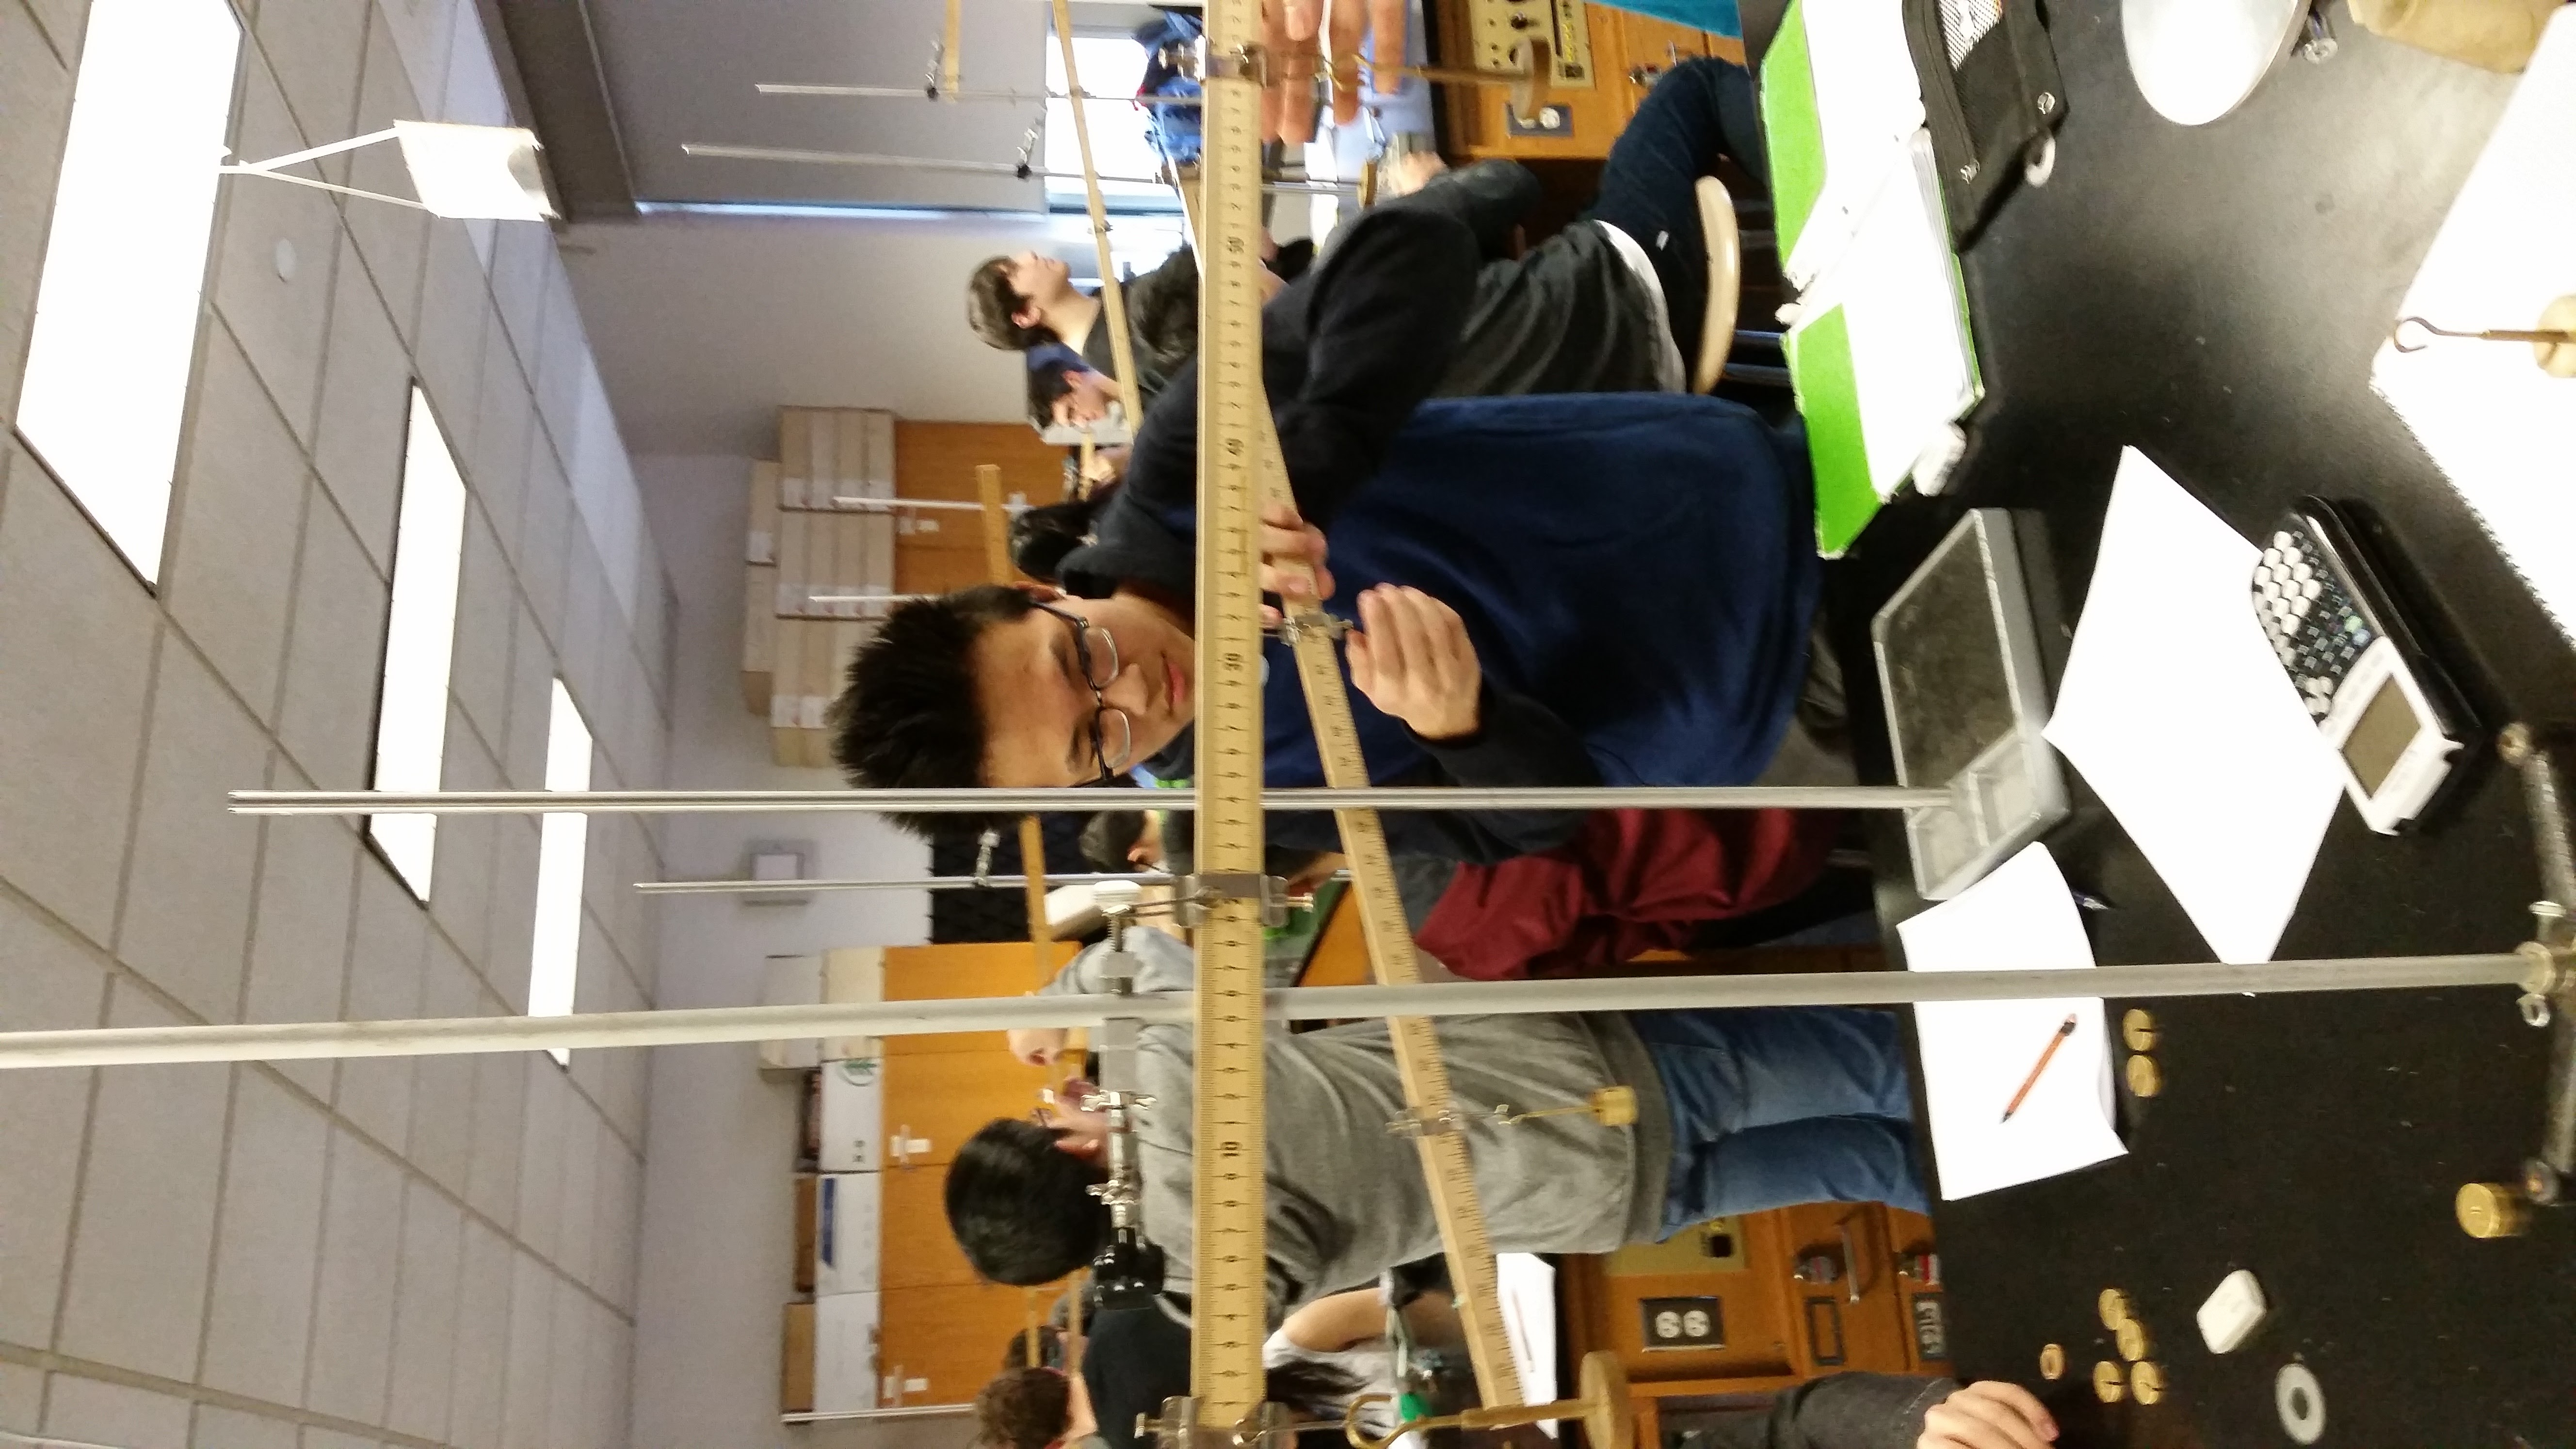
\includegraphics[scale=0.15, angle=270]{lab4.jpg}
\vspace*{19cm}
\end{figure}

\begin{center}
\begin{tabular}
{|m{7em}|m{7em}|}
\hline
\hline
\end{tabular}

\section*{Discussion}
Sample calculations for the non-measured data are as shown:

\section*{Conclusion}


\end{document}
